\section{Experiments}
\label{sec:experiments}

Our experimental analysis addresses five questions:
(1) How does CORELS' accuracy compare to other algorithms?
(2) How does CORELS' model size compare to other algorithms?
(3) How rapidly does the objective function converge?
(4) How rapidly does CORELS prune the search space?
(5) How much does each of the implementation optimizations contribute to CORELS' performance?

\subsection{Computational environment}

All results that we present were executed on a server with two Intel Xeon E5-2699~v4
(55~MB cache, 2.20~GHz) processors and 448~GB RAM.
%
Except where we mention a memory constraint, all experiments
can run comfortably on smaller machines, \eg a laptop with 16GB~RAM.

\subsection{Datasets and prediction problems}

Our evaluation focuses on two socially-important prediction problems associated
with recent, publicly-available datasets:
\begin{itemize}
\item Predicting which individuals in the ProPublica COMPAS
dataset~\citep{LarsonMaKiAn16} recidivate within two years.
This dataset contains records for all offenders in Broward County, Florida
in 2013 and 2014 who were given a COMPAS score pre-trial.
Recidivism is defined as committing a crime within 2 years of the COMPAS
assessment.
This dataset contains records for 7,215 individuals.
%
Our rule mining framework extracts 14 features and combines them into
156 antecedents on average (folds ranged from containing 155 to 157 antecedents).
%
\item Using the NYCLU 2014 stop-and-frisk dataset~\citep{nyclu:2014} to predict
whether a weapon will be found on a stopped individual who is frisked or searched.
%
From the original dataset of 45,787 records, each describing an incident involving
a stopped person, we identify a subset of 29,595 records for which the individual
was frisked and/or searched.
%
Of these, criminal possession of a weapon was identified in only about 5\% of instances.
%
Resampling due to class imbalance, for 10-fold cross-validation, yields training sets
that each contain 50,743 datapoints.
%
From a set of 5 categorical features, we form a set of~28 single-clause antecedents
that we use in our experiments below, through~\S\ref{sec:sparsity}.
%
For our experiments in~\S\ref{sec:traces}, we add negations of 18 of these antecedents,
which gives a total of 46 antecedents.
\end{itemize}
%
For further details about data preprocessing steps and antecedent mining, see Appendix~C.
%
Our choice of and approach to the weapon prediction problem is inspired by the work
of~\citet{Goel16}, who develop regression models to analyze racial disparities
in New York City's stop-and-frisk policy, for a similar, larger dataset.
%
In particular, the authors arrive at a simple and interpretable heuristic that
could potentially help police officers more effectively decide when to
frisk and/or search stopped individuals, \ie when such
interventions are likely to discover criminal possession of a weapon.

\subsection{Example rule lists}

We first ran a 10-fold cross validation experiment using CORELS
and eight other algorithms:
logistic regression, support vector machines, AdaBoost, CART, C4.5,
random forests, RIPPER, and scalable Bayesian rule lists (SBRL).~\footnote{For
SBRL, we use the C implementation at \url{https://github.com/Hongyuy/sbrlmod}.}
%
We use standard R packages, with default parameter settings,
for the first seven algorithms.~\footnote{For CART, C4.5 (J48), and RIPPER,
\ie the tree and rule list learning algorithms, we use the implementations
from the R packages rpart, RWeka, and caret, respectively.
%
By default, CART uses complexity parameter ${cp = 0.01}$,
and C4.5 uses complexity parameter ${C = 0.25}$.
}

\begin{figure}[t]
\begin{algorithmic}
\State \bif $(age = 23-25) \band (priors = 2-3)$ \bthen $yes$
\State \belif $(age = 18-20)$ \bthen $yes$
\State \belif $(sex = male) \band (age = 21-22)$ \bthen $yes$
\State \belif $(priors > 3)$ \bthen $yes$
\State \belse $no$
\end{algorithmic}
\vspace{1mm}
\begin{algorithmic}
\State \bif $(age = 23-25) \band (priors = 2-3)$ \bthen $yes$
\State \belif $(age = 18-20)$ \bthen $yes$
\State \belif $(priors > 3)$ \bthen $yes$
\State \belif $(sex = male) \band (age = 21-22)$ \bthen $yes$
\State \belse $no$
\end{algorithmic}
\vspace{1mm}
\begin{algorithmic}
\State \bif $(age = 23-25) \band (priors = 2-3)$ \bthen $yes$
\State \belif $(sex = male) \band (age = 21-22)$ \bthen $yes$
\State \belif $(age = 18-20)$ \bthen $yes$
\State \belif $(priors > 3)$ \bthen $yes$
\State \belse $no$
\end{algorithmic}
\caption{Example optimal rule lists that predict two-year recidivism for the
ProPublica dataset, found by CORELS, across 10 cross-validation folds.
%
The most common of these was found by 6 folds (top),
the next was found by 2 folds (middle), and the last by 1 fold (bottom).
%
We observe that all of these rule lists start with the same rule,
end with the same default rule, and contain the same prefix rules, up to a permutation;
the prefix rules always predict the positive class label,
and the default rule always predicts the negative class label.
%
Note that our objective is not designed to enforce any of these properties,
though some may be seen as desirable.
}
\label{fig:recidivism-all-folds}
\end{figure}

\begin{figure}[t!]
\begin{algorithmic}
\State \bif $(location = transit~authority)$ \bthen $yes$
\State \belif $(stop~reason = suspicious~object)$ \bthen $yes$
\State \belif $(stop~reason = suspicious~bulge)$ \bthen $yes$
\State \belse $no$
\end{algorithmic}
\caption{An example rule list that predicts whether a weapon will be found on a
stopped individual who is frisked or searched, for the NYCLU stop-and-frisk dataset.
%
This is the most common optimal rule list found by CORELS across 10 cross-validation
folds; the others contain the same rules, up to a permutation.
}
\label{fig:weapon-rule-list}
\end{figure}

\begin{figure}[t!]
\begin{center}
%\includegraphics[width=0.75\textwidth]{figs/sketch-comparison.png}
% left lower right upper
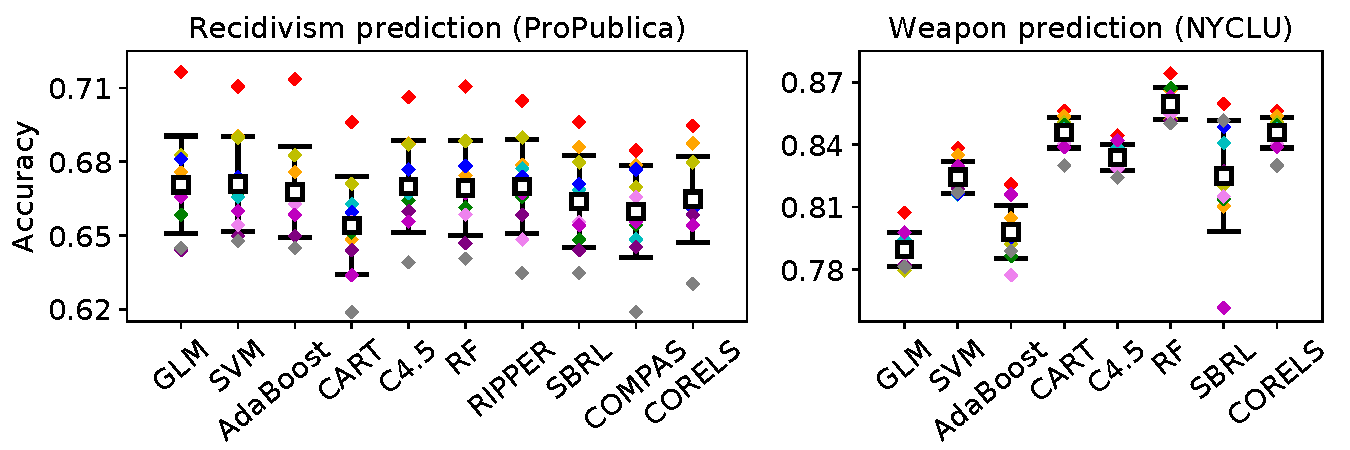
\includegraphics[trim={14mm, 5mm, 30mm, 5mm},
width=\textwidth]{figs/compare-compas-weapon.pdf}
\end{center}
\caption{Comparison of CORELS and a panel of eight other algorithms:
logistic regression~(GLM), support vector machines~(SVM),
AdaBoost, CART, C4.5, random forests~(RF), RIPPER,
scalable Bayesian rule lists~(SBRL).
%
Test accuracy means (white squares),
standard deviations (error bars),
and values (colors correspond to folds),
for 10-fold cross-validation experiments.
%
Left:~Two-year recidivism prediction for the ProPublica COMPAS dataset.
%
For CORELS, we use regularization parameter~${\Reg=0.005}$.
%
Right:~Weapon prediction for the NYCLU stop-and-frisk dataset.
%
For CORELS, we use~${\Reg=0.01}$.
%
Note that we were unable to execute RIPPER for the NYCLU problem.
}
\label{fig:comparison}
\end{figure}

Figures~\ref{fig:recidivism-all-folds} and~\ref{fig:weapon-rule-list}
show example optimal rule lists that CORELS learns
for the ProPublica and NYCLU datasets, respectively.
%
While our goal is to provide illustrative examples, and not to provide a
detailed analysis nor to advocate for the use of these specific models,
we note that these rule lists are short and easy to understand.
%
In particular, the three-rule list for weapon prediction
in Figure~\ref{fig:weapon-rule-list} has the spirit of the heuristic
strategy presented by~\citet{Goel16} that combines three stop criteria
and is based on a reduced version of their full regression model.

\subsection{Comparison of accuracy and model size for CORELS and other algorithms}
\label{sec:sparsity}

Figure~\ref{fig:comparison} shows that there were no statistically significant
differences in algorithm accuracies.
In fact, the difference between folds was far larger than the difference
between algorithms.
We conclude that CORELS produces models whose accuracy is comparable
to those found via other algorithms.

\begin{figure}[t!]
\begin{center}
%\includegraphics[width=0.75\textwidth]{figs/sketch-comparison.png}
% left lower right upper
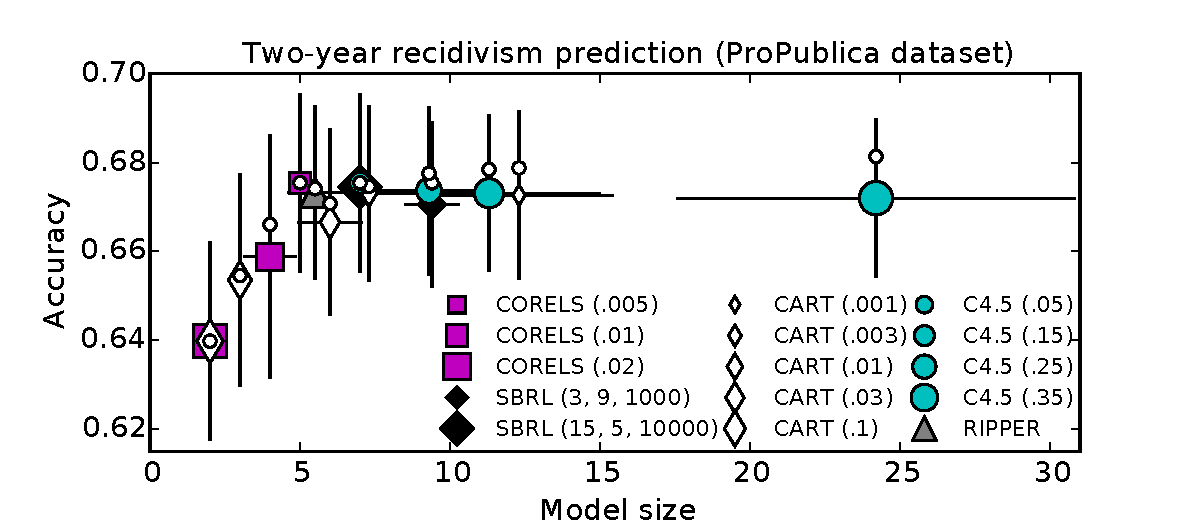
\includegraphics[trim={12mm, 0mm, 24mm, 5mm},
width=0.9\textwidth]{figs/compas-sparsity-training.pdf}
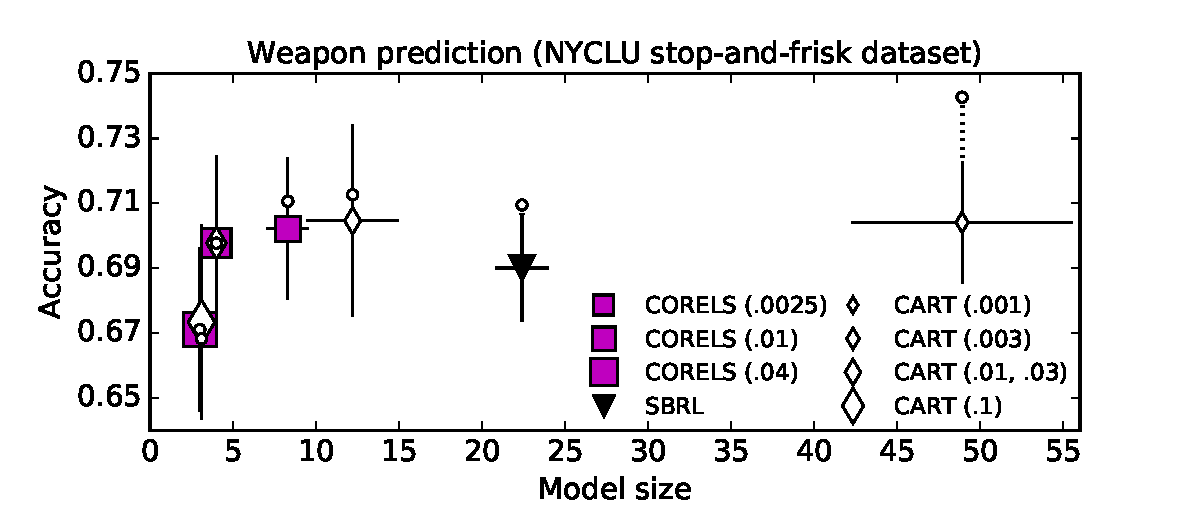
\includegraphics[trim={12mm, 0mm, 24mm, 1mm},
width=0.9\textwidth]{figs/frisk-sparsity-training.pdf}
\end{center}
\caption{Training and test accuracy as a function of model size.
%
For CORELS, CART, and C4.5, we vary the regularization parameter~$\Reg$,
and complexity parameters~$cp$ and~$C$, respectively;
numbers within parentheses in the legend indicate parameter values.
%
Note that the CART implementation sets ${cp = 0.01}$ by default,
and C4.5 uses ${C = 0.25}$.
%
Legend markers and error bars indicate means and standard deviations,
respectively, of test accuracy across cross-validation folds.
%
Small circles mark associated training accuracy means.
%
Top:  Two-year recidivism prediction for the ProPublica COMPAS dataset.
%
None of the models exhibit significant overfitting --
mean training accuracy never exceeds mean test accuracy
by more than about 0.01.
%
Bottom:  Weapon prediction for the NYCLU stop-and-frisk dataset.
%
Only CART with ${cp = 0.001}$ significantly overfits.
%
We do not depict C4.5, which finds large models (${>100}$ leaves)
and dramatically overfits for all tested parameters.
}
\label{fig:sparsity}
\end{figure}

Figure~\ref{fig:sparsity} summarizes differences in accuracy and model size
for CORELS and other tree (CART, C4.5) and rule list (RIPPER, SBRL) learning algorithms.
%
For both problems, CORELS can learn short rule lists without sacrificing accuracy.

\begin{figure}[t!]
\begin{center}
%\includegraphics[width=0.65\textwidth]{figs/sketch-objective.png}
% left lower right upper
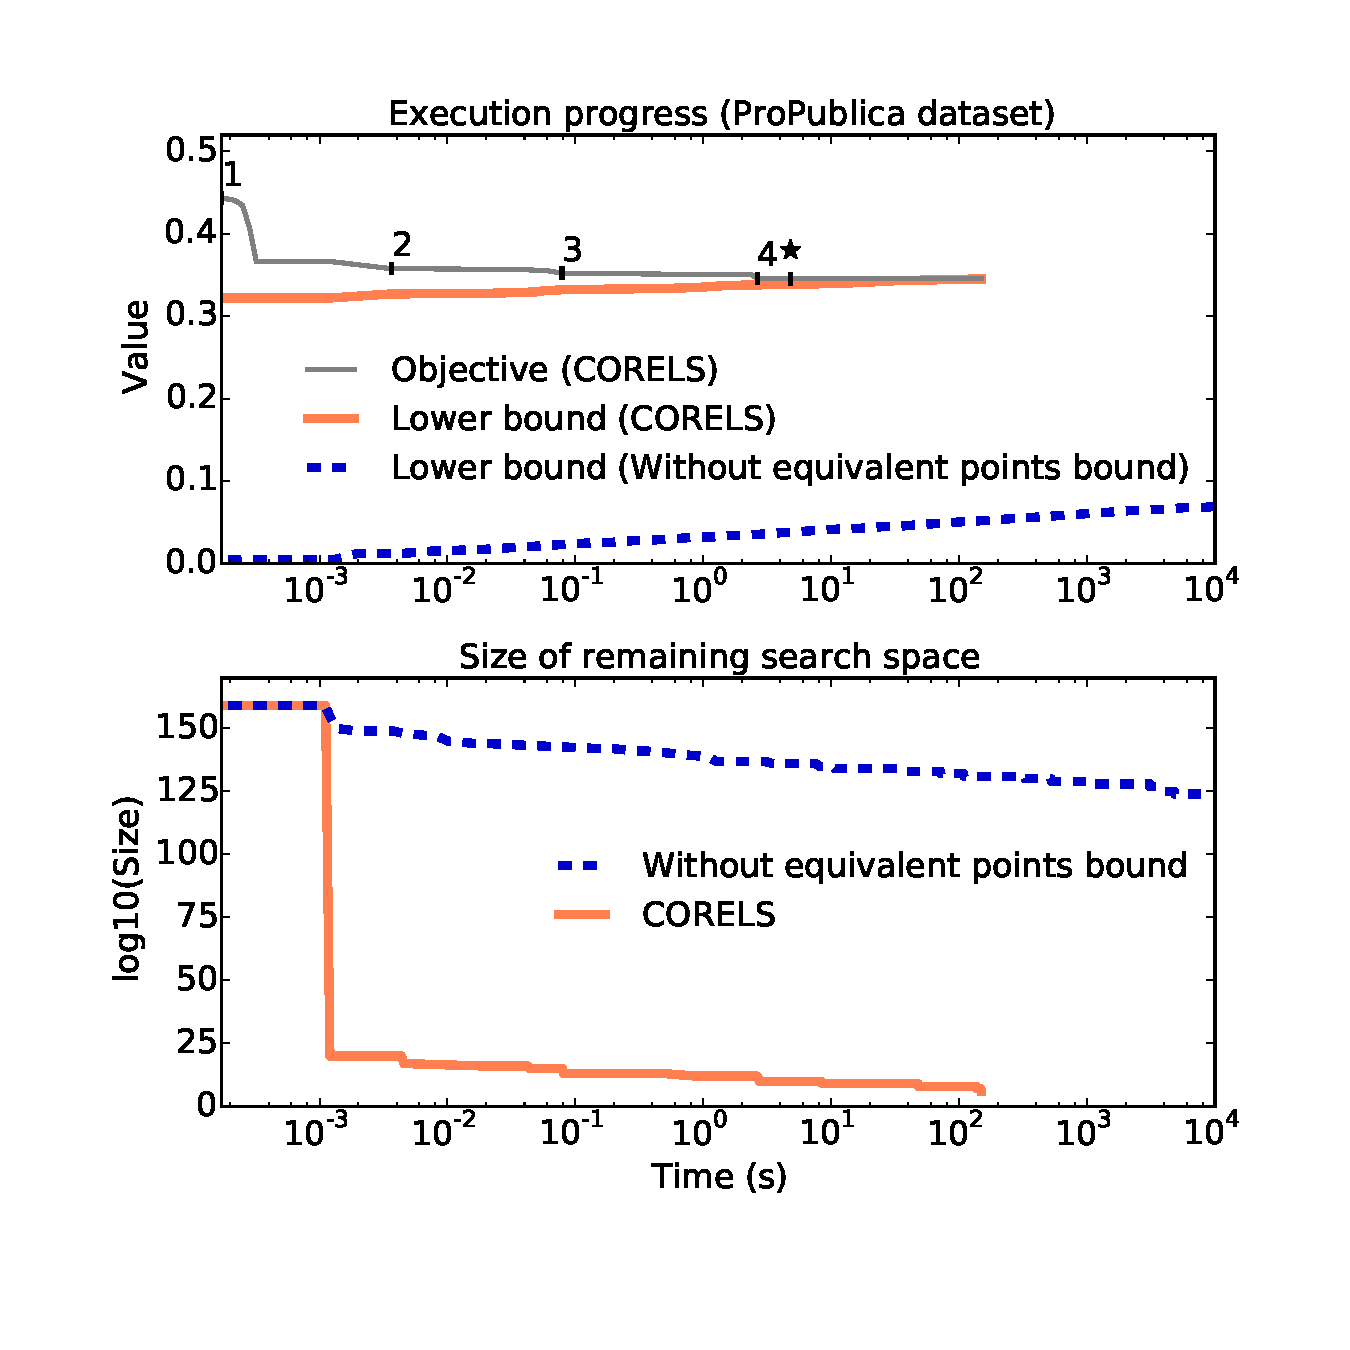
\includegraphics[trim={20mm, 25mm, 24mm, 20mm},
width=0.9\textwidth]{figs/compas_execution_large-remaining-space.pdf}
\end{center}
\caption{CORELS with (lines) and without
(dashes) the equivalent points bound (Theorem~\ref{thm:identical}),
for the ProPublica dataset.
%
Top: Objective value (thin line) and lower bound (thick line) for CORELS,
as a function of wall clock time (log scale).
%
Numbered hatch marks along the trace of the objective value
indicate when the length of the best known rule list changes,
and are labeled by the new length.
%
CORELS quickly achieves the optimal value (star marker),
and certifies optimality when the lower bound matches the objective value.
%
A separate execution of CORELS without the equivalent points (Theorem~\ref{thm:identical})
bound remains far from complete, and its lower bound (dashed line) far from the optimum.
%
Bottom: $\lfloor \log_{10} \Remaining(\CurrentObj, \Queue) \rfloor$,
as a function of wall clock time (log scale),
where~$\Remaining(\CurrentObj, \Queue)$
is the upper bound on remaining search space size
(Theorem~\ref{thm:remaining-eval-fine}).
%
For this problem, the equivalent points bound is responsible for the ability of
CORELS to quickly eliminate most of the search space (solid line);
the remaining search space decays much more slowly without this bound (dashed line).
}
\label{fig:objective}
\end{figure}

\subsection{CORELS execution traces and efficacy of algorithm optimizations}
\label{sec:traces}

In the remainder, we show results using the ProPublica dataset.
%
The solid lines in Figure~\ref{fig:objective} illustrate how both the objective (top)
and the size of the remaining search space (bottom) decrease as CORELS executes.
%
The objective drops quickly, achieving the optimal value within 10 seconds.
CORELS certifies optimality in less than 6 minutes --
the objective lower bound of the remaining search space
steadily converges to the optimal objective as the search space shrinks.

Finally, we determine the efficacy of each of our bounds and data structure optimizations.
%
Both panels of Figure~\ref{fig:objective} additionally highlight a separate
execution of CORELS without the equivalent points bound.
%
After nearly 3 hours, the execution is still far from complete;
in particular, the lower bound is far from the optimum objective value.
%
Table~\ref{tab:ablation} provides summary statistics for experiments using the full
CORELS implementation and five variants that each remove a specific optimization.
%
Figure~\ref{fig:queue} presents a view of the same experiments.
%
These plots depict the number of prefixes of a given length in the queue
during the algorithm's execution.

%\includegraphics[width=0.75\textwidth]{figs/sketch-ablation.png}
\begin{table}[t!]
\begin{tabular}{l | c  r | c | c}
& Total time & Slow- & Time to & Max evaluated~ \\
Algorithm variant & (min) & down & optimum (s) & prefix length \\
\hline
CORELS & 5.5 (1.6) & --- & 8 (2) & 5-6 \\
No priority queue (BFS) & 6.8 (2.2) & 1.2$\times$ & 4 (1) & 5-6 \\
No support bounds & 10 (3.4) & 1.8$\times$ & 13 (4) & 5-6 \\
No symmetry-aware map & 59 (23) & 10$\times$ & 23 (6) & 5-6 \\
No lookahead bound & 72 (23) & 13$\times$ & 9 (2) & 6-7 \\
No equivalent points bound & $>$190 (100) & $>$39$\times$ & $>$7100~* & $\ge$10 \\
\hline
\end{tabular}
\begin{tabular}{l | c | c | c}
\hline
 & Lower bound & Total queue &  Max queue \\
Algorithm variant & evaluations ($\times 10^6$) & insertions ($\times 10^6$) & size ($\times 10^6$) \\
\hline
CORELS & 180 (54) & 1.7 (0.4) & 1.3 (0.4) \\
No priority queue (BFS) & 230 (75) & 1.9 (0.6) & 1.5 (0.5) \\
No support bounds & 360 (120) & 2.7 (0.8) & 2.2 (0.7) \\
No symmetry-aware map & 2000 (770) & 16 (5.9) & 15 (5.7) \\
No lookahead bound & 2200 (710) & 19 (5.9) & 16 (5.3) \\
No equivalent points bound & $>$1490 & $>$800 & $>$790 \\
\end{tabular}
%\vspace{4mm}
\caption{Per-component performance improvement.
%
The columns report the total execution time,
time to optimum, maximum evaluated prefix length,
number of times we completely evaluate a prefix~$\Prefix$'s lower bound~$b(\Prefix, \x, \y)$,
total number of queue insertions (which is equal to the number of cache insertions),
and maximum logical queue size.
%
The first row shows CORELS; subsequent rows show variants
that each remove a specific implementation optimization or bound.
%
(We are not measuring the cumulative effects of removing a sequence of components.)
%
All rows represent complete executions, except for the final row,
in which each execution was terminated due to memory constraints,
once the size of the cache reached ${8 \times 10^8}$ elements,
after consuming 390-410GB RAM.
%
In all but the final row and column, we report means
(and standard deviations) over 10 cross-validation folds.
%
We also report the  mean slowdown in total execution time,
with respect to CORELS.
%
In the final row, we report the mean (and standard deviation) of the
incomplete execution time and corresponding slowdown;
in the remaining fields, we report minimum values across folds.
%
*~Only 4 out of 10 folds achieve the optimum before being terminated.
}
\vspace{4mm}
\label{tab:ablation}
\end{table}

\begin{table}[t!]
\begin{tabular}{l | c  r | c | c}
& Total time & Slow- & Time to & Max evaluated~ \\
Algorithm variant & (s) & down & optimum ($\mu$s) & prefix length \\
\hline
CORELS & 47.43 (3.8) & 1.00$\times$ & 0 (0) & 11-11 \\
No priority queue (BFS) & 143.71 (13.0) & 3.03$\times$ & 0 (0) & 11-11 \\
No support bounds & 89.58 (7.6) & 1.89$\times$ & 0 (0) & 11-12 \\
No symmetry-aware map & 2697.78 (8093.3) & 66.63$\times$ & 0 (0) & 1-11 \\
No lookahead bound & 75.14 (5.2) & 1.59$\times$ & 0 (0) & 11-12 \\
No equivalent points bound & 0.00 (0.0) & 0.00$\times$ & 0 (0) & 1-1 \\
\hline
\end{tabular}
\begin{tabular}{l | c | c | c}
\hline
 & Lower bound & Total queue &  Max queue \\
Algorithm variant & evaluations ($\times 10^5$) & insertions ($\times 10^5$) & size ($\times 10^5$) \\
\hline
CORELS & 64.58 (4.9) & 1.73 (0.1) & 1.13 (0.1) \\
No priority queue (BFS) & 200.73 (17.5) & 5.40 (0.5) & 2.00 (0.1) \\
No support bounds & 121.54 (9.8) & 3.08 (0.3) & 1.91 (0.1) \\
No symmetry-aware map & 3891.73 (11675.2) & 107.35 (322.0) & 79.87 (239.6) \\
No lookahead bound & 102.41 (7.3) & 2.78 (0.2) & 1.82 (0.1) \\
No equivalent points bound & 0.00 (0.0) & 0.00 (0.0) & 0.00 (0.0) \\
\end{tabular}
%\vspace{4mm}
\caption{Per-component performance improvement.
%
The columns report the total execution time,
time to optimum, maximum evaluated prefix length,
number of times we completely evaluate a prefix~$\Prefix$'s lower bound~$b(\Prefix, \x, \y)$,
total number of queue insertions (which is equal to the number of cache insertions),
and maximum logical queue size.
%
The first row shows CORELS; subsequent rows show variants
that each remove a specific implementation optimization or bound.
%
(We are not measuring the cumulative effects of removing a sequence of components.)
%
All rows represent complete executions.
%
We report means (and standard deviations) over 10 cross-validation folds.
%
We also report the  mean slowdown in total execution time,
with respect to CORELS.
}
\vspace{4mm}
\label{tab:ablation-weapon}
\end{table}

\begin{figure}[t!]
\begin{center}
% left lower right upper
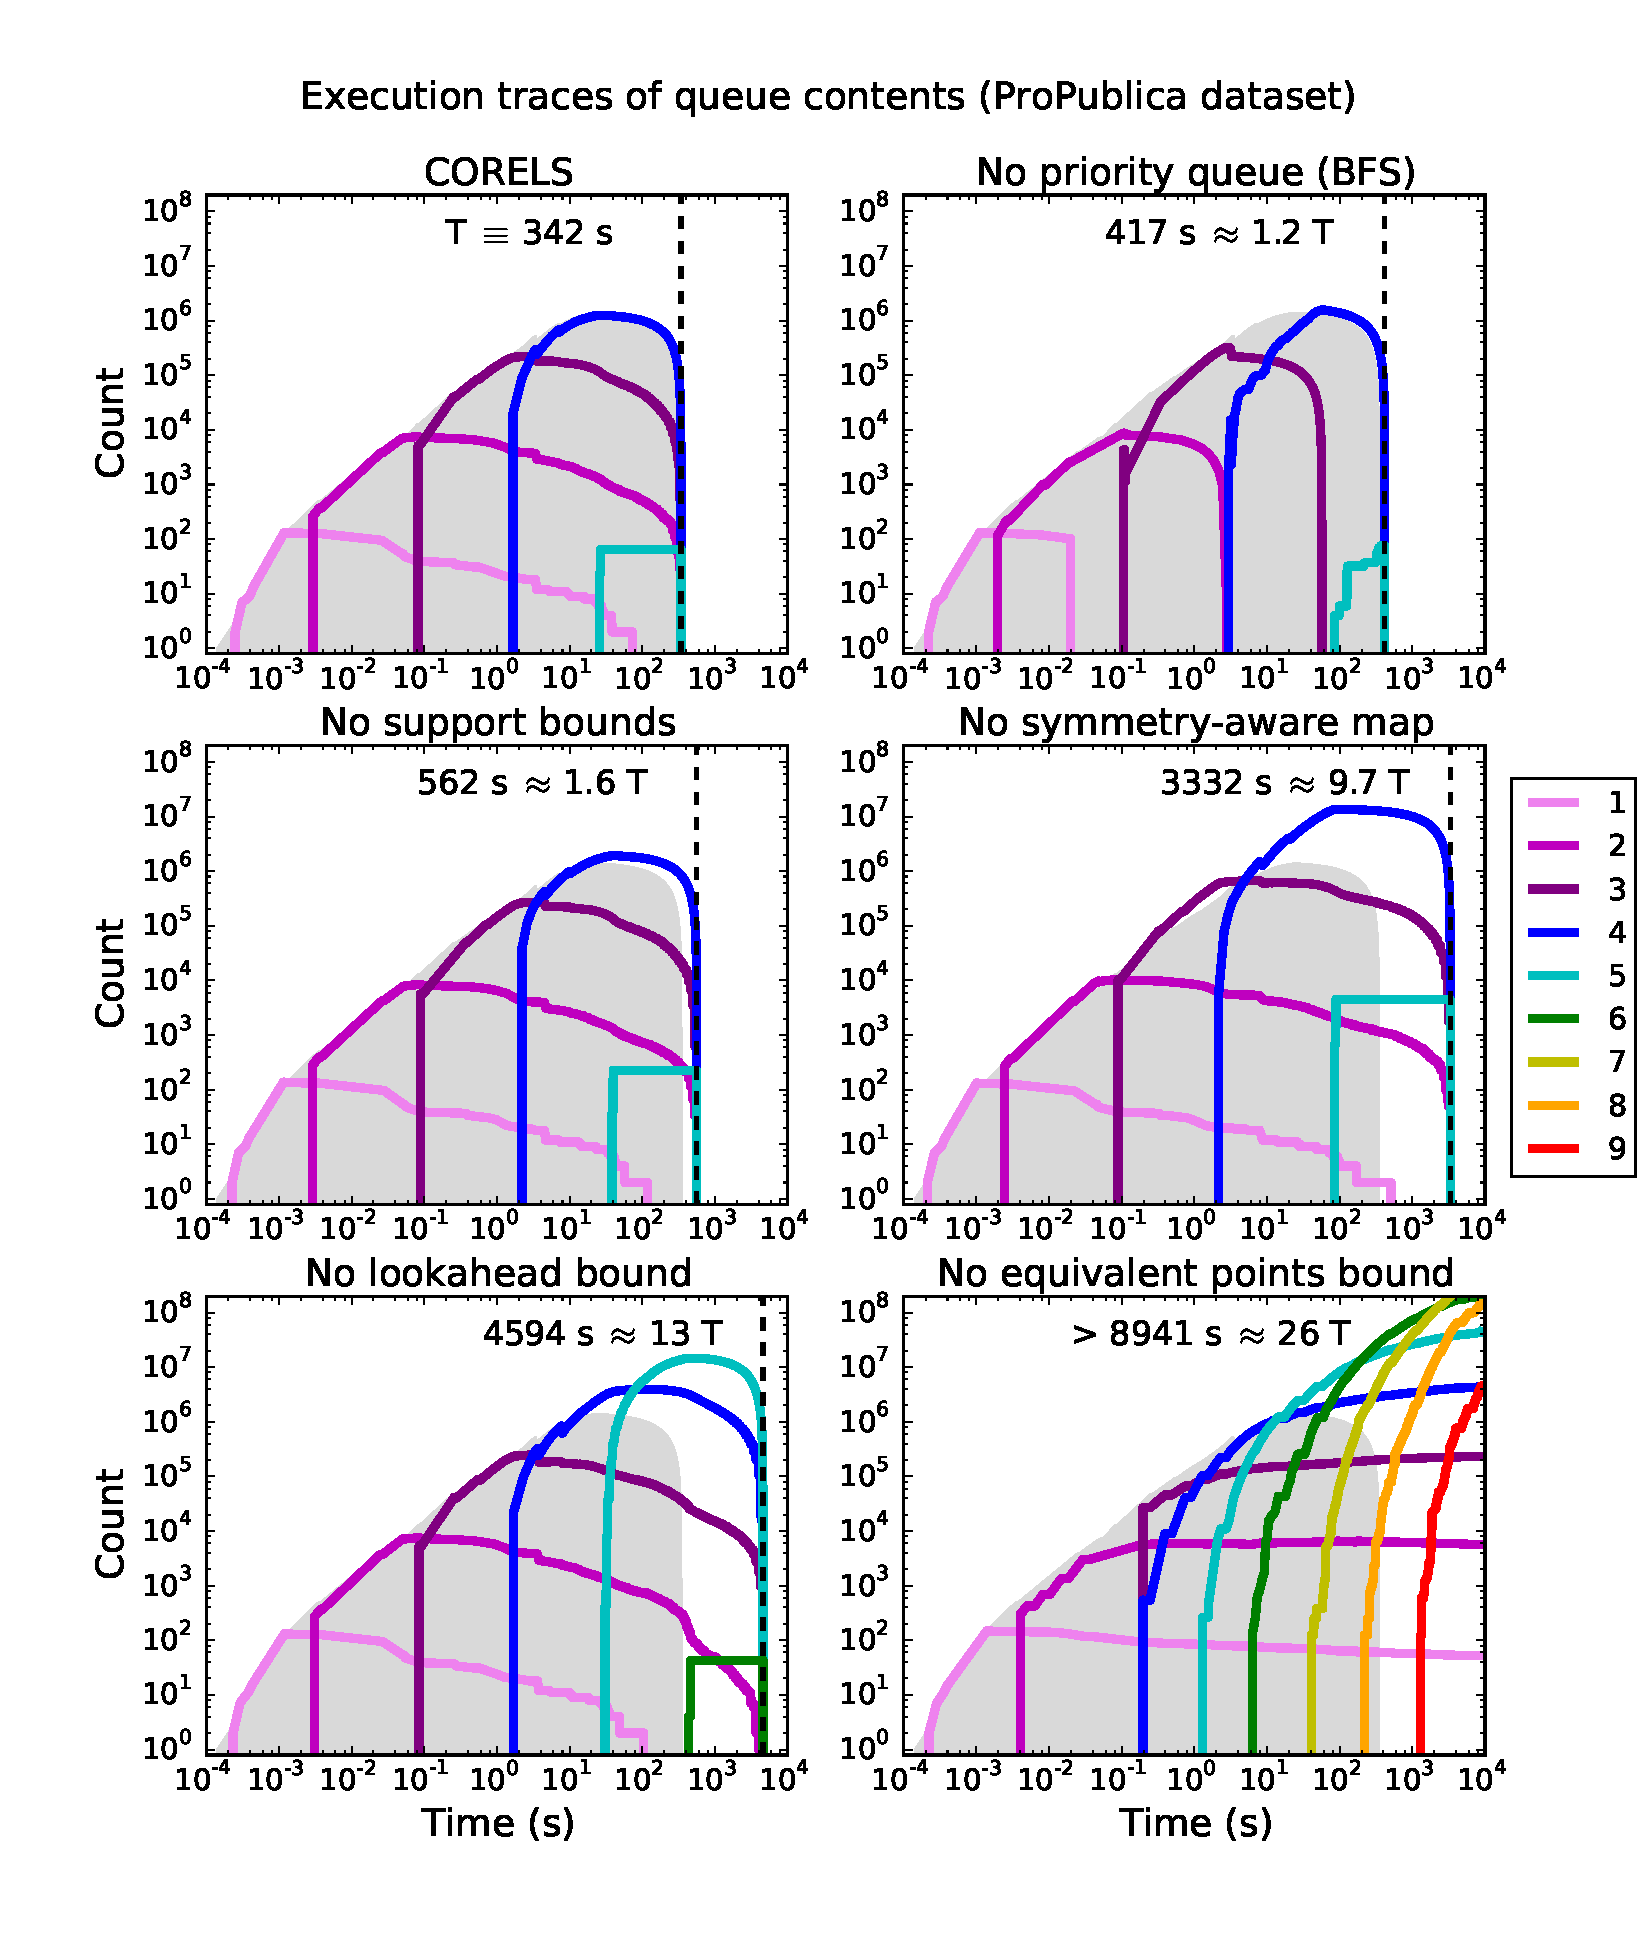
\includegraphics[trim={15mm 20mm 5mm 25mm},
width=0.94\textwidth]{figs/kdd_compas_ablation-queue.pdf}
\end{center}
\vspace{-5mm}
\caption{Summary of the logical queue's contents, for full CORELS (top left)
and five variants that each remove a specific implementation optimization or bound,
as in Table~\ref{tab:ablation}.
%
%We summarize the composition of the logical queue,
%\ie the nodes in the physical that have not been marked for deletion.
%
Solid lines plot the numbers of prefixes in the logical queue (log scale), colored by length (legend),
as a function of wall clock time (log scale).
%
All plots are generated using a single, representative cross-validation training set.
%
%EXPAND HERE
%the permutation bounds (top right),
%lookahead bound (bottom left), and equivalent points bound (bottom right).
%
The gray shading fills in the area beneath the total number of
queue elements for CORELS,
\ie the sum over all lengths in the top left figure.
%
For comparison, we replicate the same gray region
in the other five subfigures.
%
For each execution, we indicate the total time in seconds,
relative to the full CORELS implementation (T = 342 s),
and with a dashed vertical line.
%
Note that the execution without the equivalent points bound (bottom right) is incomplete.
}
\label{fig:queue}
\end{figure}

\begin{figure}[t!]
\begin{center}
% left lower right upper
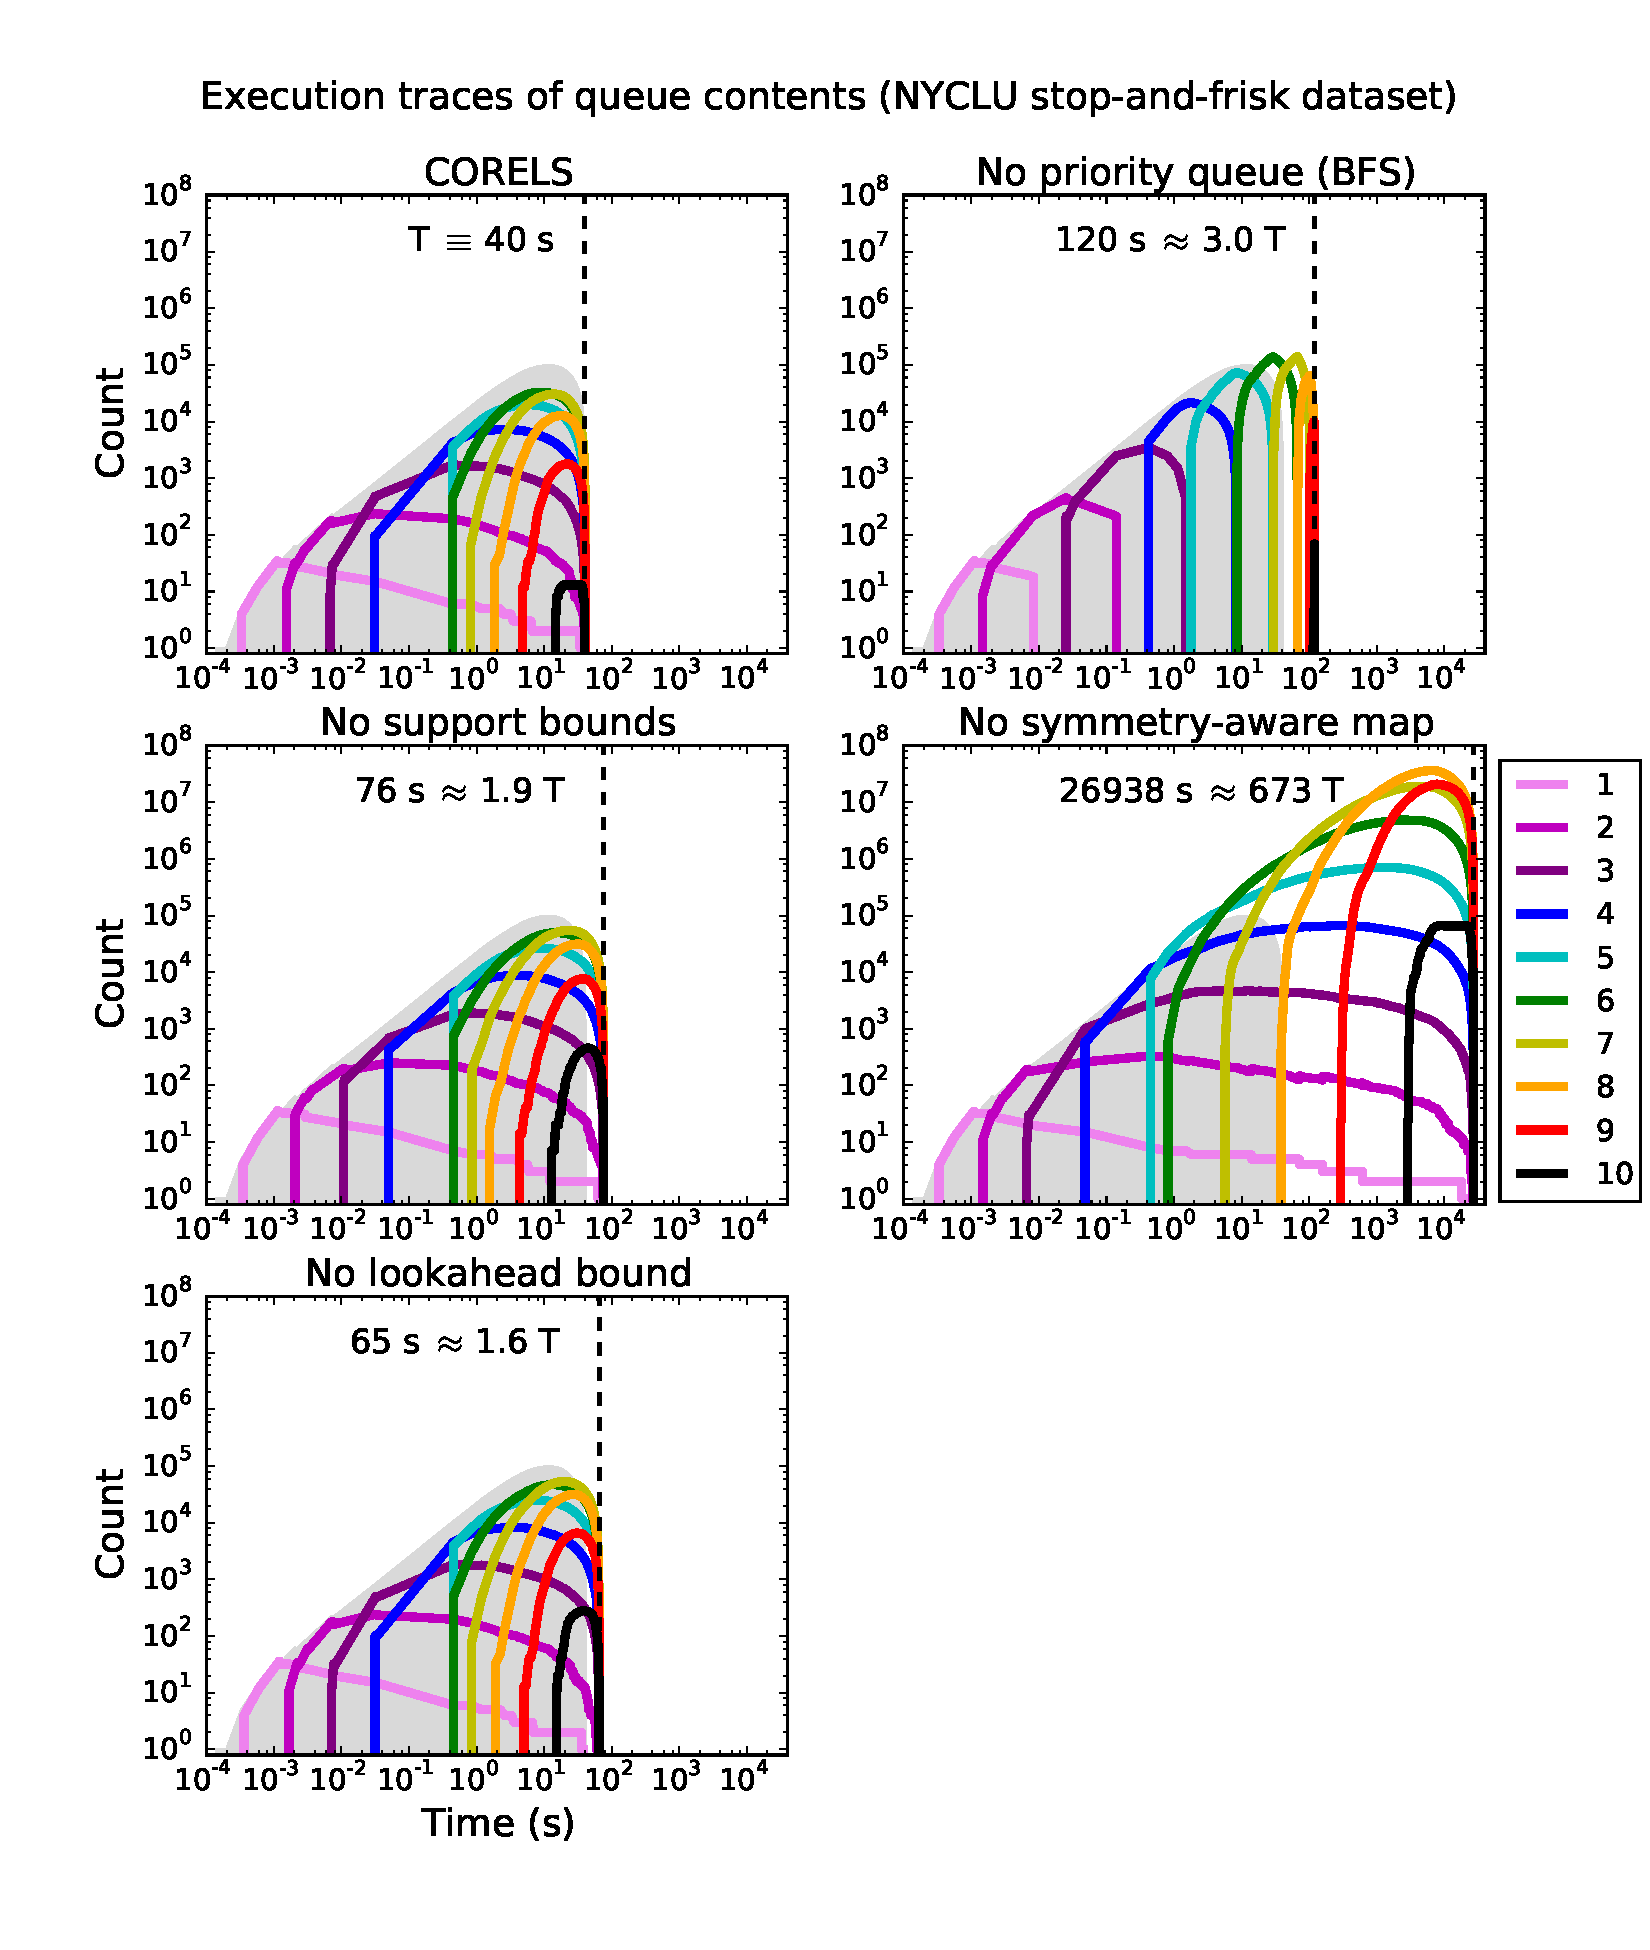
\includegraphics[trim={15mm 20mm 5mm 25mm},
width=0.94\textwidth]{figs/weapon_ablation-queue.pdf}
\end{center}
\vspace{-5mm}
\caption{Summary of the logical queue's contents, for full CORELS (top left)
and five variants that each remove a specific implementation optimization or bound,
as in Table~\ref{tab:ablation}.
%
%We summarize the composition of the logical queue,
%\ie the nodes in the physical that have not been marked for deletion.
%
Solid lines plot the numbers of prefixes in the logical queue (log scale), colored by length (legend),
as a function of wall clock time (log scale).
%
All plots are generated using a single, representative cross-validation training set.
%
%EXPAND HERE
%the permutation bounds (top right),
%lookahead bound (bottom left), and equivalent points bound (bottom right).
%
The gray shading fills in the area beneath the total number of
queue elements for CORELS,
\ie the sum over all lengths in the top left figure.
%
For comparison, we replicate the same gray region
in the other five subfigures.
%
For each execution, we indicate the total time in seconds,
relative to the full CORELS implementation (T = 40 s),
and with a dashed vertical line.
}
\label{fig:queue-weapon}
\end{figure}

\subsection{Algorithmic Speedup}
%TODO Remove calculation
We calculate the overall speed-up of CORELS compared to a naive implementation and determine the feasibility of running
our algorithm 30 years ago.
%
On the COMPAS dataset, where the number of rules is $M = 156$, naively evaluating all prefixes of up to length 5 would
require examining $8.7 \times 10^{10}$ different prefixes.
%
However, while CORELS only examines prefixes up to length 5 in order to certify optimality, a naive implementation 
would have to look at even longer prefixes. 
%
Without our equivalent points bound, but with all of our other optimizations, we evaluate prefixes up to at least length 10 
(see \ref{tab:ablation} and \ref{fig:queue}).
%
Naively evaluating all prefixes up to length 10 would require looking at $6.4 \times 10^{21}$ different prefixes.
%
However, CORELS examines only 181,481,555 prefixes in total---a reduction of $3.5 \times 10^{13}$.
%
It takes us about 2$\mu$s to evaluate a single prefix.
%
A naive solution would take $1.54 \times 10^8$ seconds---about 5 years---while CORELS takes only 2 minutes.
%
It is clear that brute force would not scale to larger problems.
%


In addition, Moore's law holds that computing power doubled every 18 months from 1984-2006.
%
This is a period of 264 months, which means computing power has gone up by at least a factor of $30,000$ since 1984.
%
Thus, even with our algorithmic and data structural improvements, CORELS would have run in over 3,600,000s in 1984---an unreasonable amount of time.
%
Our advances are only meaningful because we can run them on a modern system.
%
Combining our algorithmic improvements with the increase in modern processor speeds, our algorithm runs more than $10^{18}$ times faster than a naive implementation would have in 1984.
%
This helps explain why our algorithm, nor other branch-and-bound variants, had not been developed before now.